
\subsection*{6.3 Probability Calculations from Various Graphs}
Probability can be estimated from different types of graphical representations, including pie charts, histograms, cumulative frequency graphs, and Venn diagrams.

\textbf{Examples:}

\begin{flushleft}
	\textbf{Example 1: Probability from a Pie Chart}
	\begin{center}
		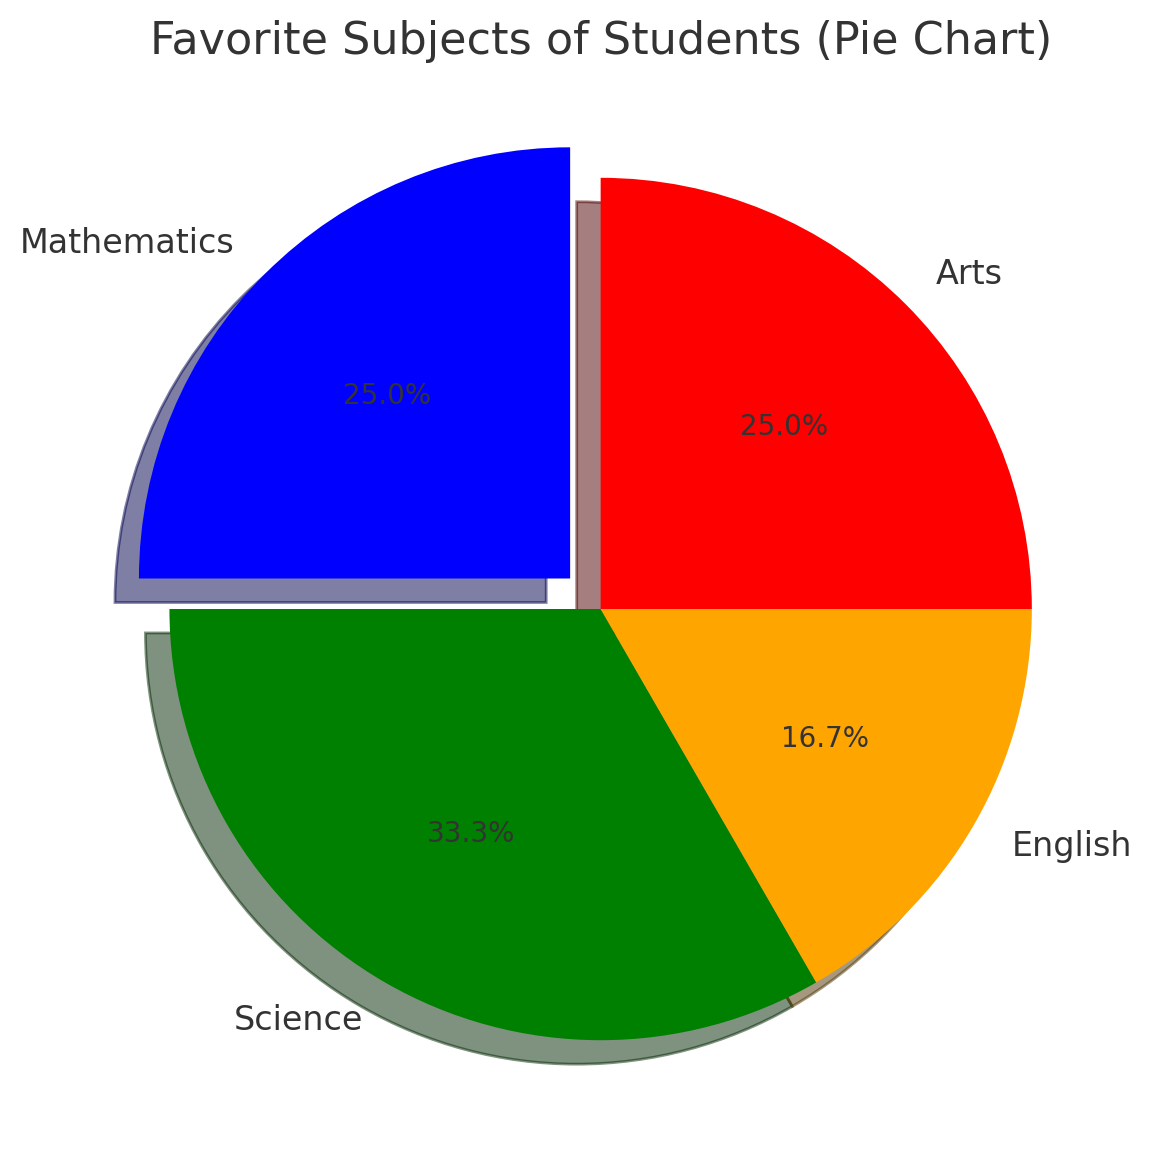
\includegraphics[width=0.6\textwidth]{6.2.png}
	\end{center}
	
	A pie chart represents the distribution of students in a school by their favorite subjects: Mathematics (90°), Science (120°), English (60°), and Arts (90°). What is the probability that a randomly chosen student prefers Science?
	
	\textbf{Solution:}
	
	Step 1: Compute the proportion of students who prefer Science.
	\[
	\text{Fraction of Science} = \frac{120^\circ}{360^\circ} = \frac{1}{3}.
	\]
	
	Step 2: Compute probability.
	\[
	P(\text{Science}) = \frac{1}{3} = 0.333.
	\]
	
	Thus, the probability that a randomly chosen student prefers Science is **$0.333$ or $33.3\%$**.
\end{flushleft}

\begin{flushleft}
	\textbf{Example 2: Probability from a Histogram}
	\begin{center}
		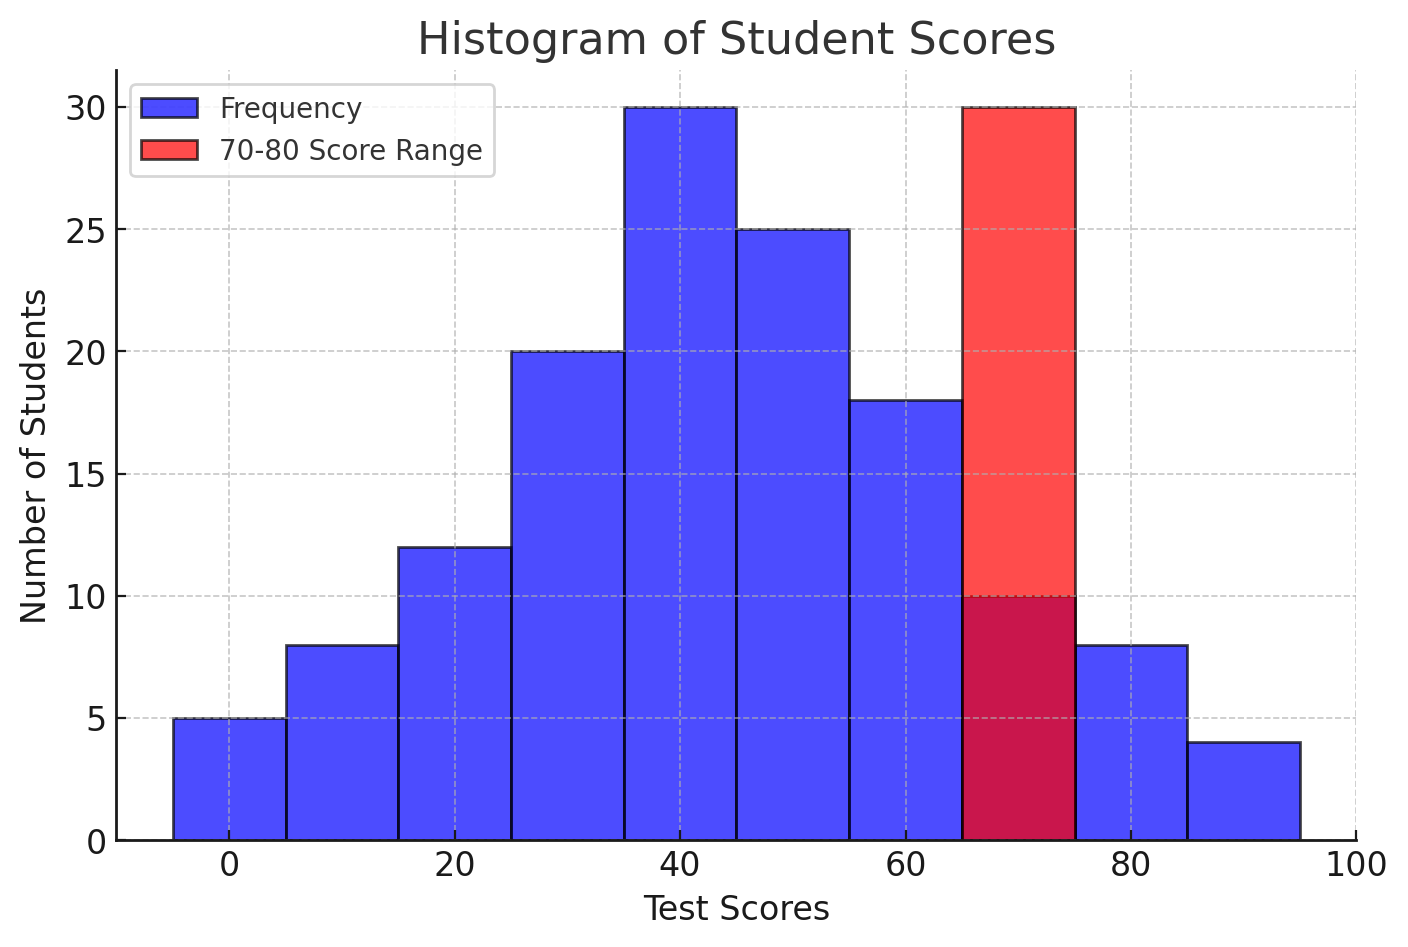
\includegraphics[width=0.6\textwidth]{6.3.png}
	\end{center}
	
	
	A histogram represents the number of students who scored different marks in a test. The total number of students is 100. Find the probability that a randomly chosen student scored between 70 and 80.
	
	\textbf{Solution:}
	
	Step 1: Use the probability formula.
	\[
	P(70 \leq \text{Score} \leq 80) = \frac{\text{Number of students in range}}{\text{Total students}}.
	\]
	
	\[
	= \frac{30}{100} = 0.30.
	\]
	
	Thus, the probability is **$0.30$ or $30\%$**.
\end{flushleft}

\begin{flushleft}
	\textbf{Example 3: Probability from a Cumulative Frequency Curve}
	
	A cumulative frequency graph shows the number of students scoring below certain marks in a test. Find the probability for the student to get distinction for the test if distinction score is 90. 
	\begin{center}
		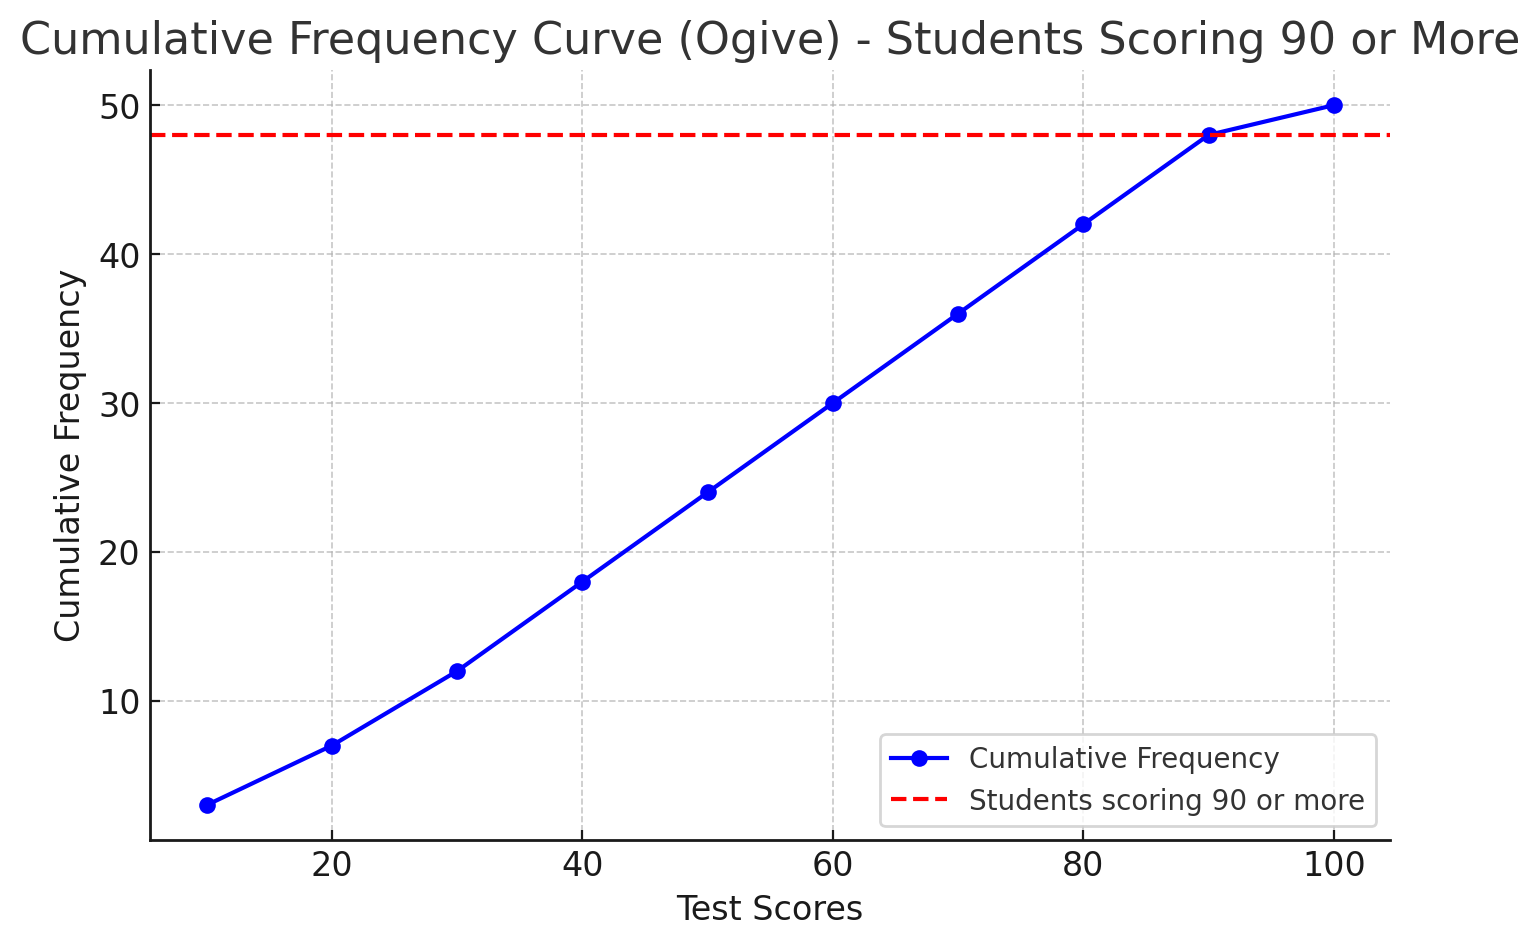
\includegraphics[width=0.6\textwidth]{6.4.png}
	\end{center}
	
	\textbf{Solution:}
	
	Step 1: Compute probability.
	\[
	P(distinction)=P(\text{Score} >90) = \frac{2}{50} = 0.04.
	\]
	
	Thus, the probability is **$0.04$ or $4\%$**.
\end{flushleft}

\begin{flushleft}
	\textbf{Example 4: Probability from a Venn Diagram}
	\begin{center}
		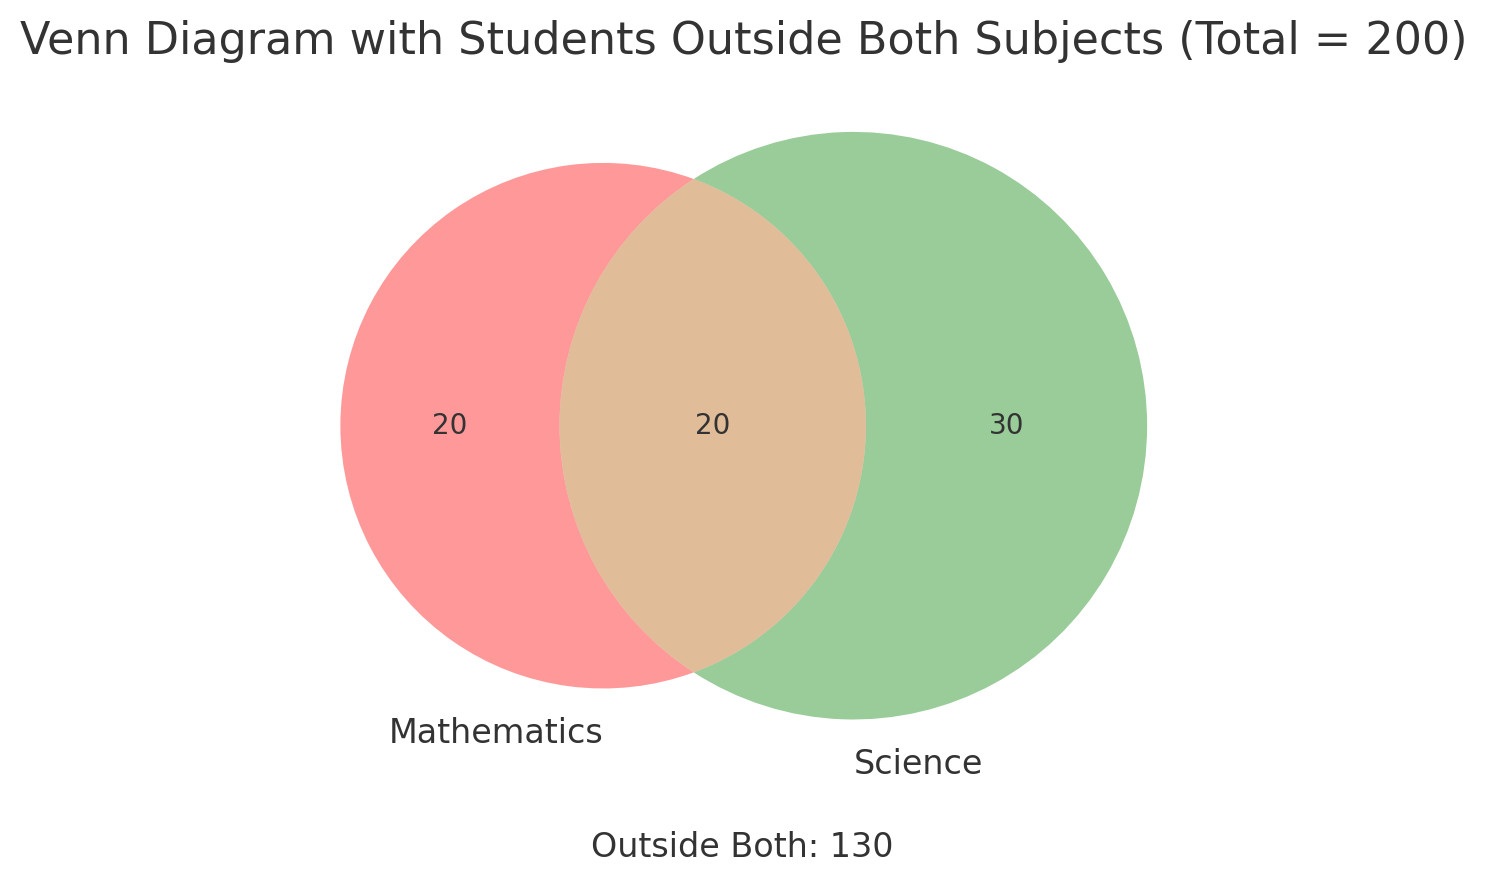
\includegraphics[width=0.6\textwidth]{6.5.png}
	\end{center}
	A Venn diagram shows the distribution of students who study Mathematics (40 students) and Science (50 students), with 20 students studying both subjects. Total number of studnets is 200. If a student is randomly selected, find \\
	a)the probability that the student studies either Mathematics or Science.\\
	b)the probability the study math only
	
	\textbf{Part A Solution:}
	
	Step 1: Use the addition rule.
	\[
	P(A \cup B) = P(A) + P(B) - P(A \cap B).
	\]
	
	\[
	P(\text{Math or Science}) = \frac{40}{200} + \frac{50}{200} - \frac{20}{100}.
	\]
	
	\[
	= \frac{70}{200} = 0.35.
	\]
	
	Thus, the probability is **$0.35$ or $35\%$**.\\
	\vspace{10pt}
	\textbf{Part B Solution:}
	\[
	P(\text{Math Only}) = \frac{20}{200}=0.1.
	\]
	Thus, the probability is **$0.10$ or $10\%$**.
	
\end{flushleft}
